A dolgozat témájának megértéséhez először meg kell vizsgálni néhány alapfogalmat, amelyek a dolgozatban szereplő rendszerekhez kapcsolódnak. Itt bemutatásra kerülnek a klasszikus tömegközlekedési rendszerek és a modernebb Intelligens Közlekedési Rendszerek (ITS)\footnote{Intelligent Transport System}, valamint a jelenleg elérhető megoldások, mint a Moovit és a Budapest Go alkalmazások, amelyek a városi közlekedés digitalizálására törekednek. Mindezek előtt azonban érdemes megvizsgálni a tömegközlekedés használatának pozitív hatásait, hogy megértsük, miért is fontos ezzel foglalkozni.

Manapság már mindenki tapasztalja a globális felmelegedés és a környezetszennyezés hatásait, amelyek egyik fő oka a közlekedési eszközök károsanyag kibocsátása. Egy 2018-as felmérés szerint a közlekedési szektor tette ki a globális szén-dioxid kibocsátás 25\%-át, ennek pedig túlnyomó része a közúti közlekedésből származik \cite{cropper2024measuring}. A közlekedési eszközök károsanyag kibocsátásának csökkentése érdekében egyre több városban és országban támogatják a tömegközlekedés használatát, mert ezáltal csökkenthető a környezetszennyezés és a városi dugók is. Több fejlődő országban elvégzett tanulmány alátámasztja a tömegközlekedési eszközök bevezetésével csökkenő légszennyezést. Például Tajpej első metrovonalának megnyitása 5-15\%-al csökkentette a levegő CO2 tartalmát \cite{cropper2024measuring}.

A tömegközlekedés nem csak a környezetvédelem szempontjából fontos, hanem a városi forgalom csökkentésében is fontos szerepet játszik. A tömegközlekedés használata csökkentheti a városi dugókat azáltal, hogy az emberek egy járműben utaznak sok személyautó helyett, így kevesebb lesz a járművekkel elfoglalt hely mérete. Egyelőre nem sokan választják a tömegközlekedést, a kisebb kényelem miatt, de megfelelő fejlesztésekkel vonzóbbá lehet tenni azt, így csökkenthető lehet a városi forgalom és a környezetszennyezés is \cite{le2016encouraging}.

A városi tömegközlekedés javításával kapcsolatban már a 70-es években is felmerült az igény a buszok automatizált kezelésére, amely akkor a megállókban való torlódást szerette volna megoldani. Ekkor használták először a Busz Flotta Kezelés (BFM)\footnote{Bus Fleet Management} kifejezést a buszok kezelésére. Később ezt a menetrendek kezelésére is alkalmazták, amely a buszok forgalmát és a járatok menetrendjét is magában foglalta. Napjainkban további feladatokkal egészül ki a tömegközlekedés menedzsmentje, amelyek úgynevezett Intelligens Közlekedési Rendszereket (ITS) hoznak létre. Ide tartozik a balesetmegelőzés, a buszok pozícióinak követése, az energiakezelés és a fenntarthatóság is. Egyes alrendszereknek saját megnevezéseik vannak, mint például a Valós Idejű Információ (RTI)\footnote{Real Time Information}, amely az utasokat tájékoztatja valós időben a közlekedés állapotáról és az esetleges változásokról, vagy az Automatikus Jármű Helyzet (AVL)\footnote{Automatic Vehicle Location} rendszer, amely a közlekedési eszközök földrajzi pozicióit követi és ezek alapján végez számításokat. A klasszikus BFM-et kibővítve az ITS-ben található elemekkel egy olyan összetett busz kezelő rendszert kapunk, amely az alap szolgáltatások mellett, lehetővé teszi a buszok helyzeteinek valós idejű követését és az utasok számára a valós idejű információk megjelenítését, és amelynek együttes megnevezése a Dynamic Bus Fleet Management \cite{orovsnjak2020bus,polyviou2011modelling}.

Az ITS rendszerek általában a következő fő komponensekből állnak \cite{polyviou2011modelling}:
\begin{enumerate}
  \item Járműre szerelt eszközök, mint a GPS, a kamera, a szenzorok és a kommunikációs eszközök.
  \item Útmenti eszközök, mint a forgalomfigyelő kamerák és a jeladók
  \item Vezérlőközpont, amely a járművek és az útmenti eszközök adatait dolgozza fel valós időben és végez számításokat ezek alapján.
  \item Kommunikációs hálózat, amely a járművek, az útmenti eszközök és a vezérlőközpont között biztosítja az információ áramlását.
  \item Megállókban felszerelt információ jelző eszközök, amelyek az utasokat tájékoztatják a járatok állapotáról és a menetrendről.
\end{enumerate}

A buszok haladásának követésére többféle módszer is létezik, amelyek közül a legelterjedtebb a GPS alapú rendszerek használata, amelyben a buszokon levő GPS modulok határozzák meg a tartózkodási helyet és valamilyen más vezeték nélküli kommunikációs csatornán keresztül továbbítódik az adat a központi szerver felé. Sajnos a GPS működését számos tényező befolyásolhatja, mint az időjárás, vagy a műholdjel gyenge minősége. Erre jelenthet megoldást egy új technológia, amely Bluetooth Low Energy (BLE) alapú jeladókat használ, amely a GPS-hez képest pontosabb helymeghatározást tesz lehetővé, de a hatótávolsága korlátozott. Ennek lényege hogy a buszokon csak egy kis fogyasztású Bluetooth jeladó működik, amely a megállókban lévő vevőkkel kommunikál, és ezek a vevők továbbítják az adatokat a központi szerverre. Ezzel a módszerrel a buszok helyzete pontosabban meghatározható, mint a GPS alapú rendszerekben, de a hatótávolság miatt csak a megállókban lehet használni. További nehézséget jelenthet, hogy minden megállóban fel kell szerelni egy jelfeldolgozó egységet, amelyhez áramforrás is szükséges. Nagyvárosokban ez még megoldható lenne, viszont távolsági buszjáratok esetében, ahol a megállók között nagy a távolság és nincs áramforrás minden vidéki megállóban, ott a GPS-es megoldás a legoptimálisabb \cite{elijah2023transforming}.

Ilyen rendszerrel rendelkezik néhány nagyváros tömegközlekedése is, mint például a Londoni iBus, amely GPS alapú helymeghatározással és GPRS alapú adatátvitellel működik. Az iBus lehetővé teszi több mint 8000 busz valós idejű követését 30 másodperces frissítési rátával, amelyek adataiból kinyert információkat a buszokon található kijelzőkön és a megállókban is megjeleníti \cite{hounsell2012data}.

A jelenleg elérhető rendszereken még mindig lehetne fejleszteni, mert a más területek technológiai fejlődéséhez viszonyítva még mindig le van maradva a tömegközlekedés. Nagyobb a baj a kisvárosokban, ahol csak kis mértékben vagy egyáltalán nincs digitalizálva a rendszer. Ennek a helyzetnek a javításához szükség lenne egy olyan rendszerre, amely valós idejű információkat szolgáltat a járatokról, lehetővé teszi az online jegyvásárlást és az útvonaltervezést. Ehhez a buszok, vonatok és metrók különböző eszközökkel való felszerelésére van szükség, mint a jegyszkennelő automata, a kártyás fizetést biztosító POS terminál vagy a GPS modul. Egy ilyen rendszerrel való interakcióba lépéshez szükség van egy felhasználói felületre is, amely lehetővé teszi az utasok számára a különböző szolgáltatások elérését: az útvonaltervezést, a valós idejű forgalmi adatok megtekintését és a jegyvásárlást \cite{rollandinfrastrukturalis}. Erre a célra már léteznek megoldások, de ezek nem fedik le teljesen a busztársaságok igényeit és még messze állunk attól, hogy ezt minden város és busztársaság használni tudja.

\section{Létező megoldások}
Kutatásunk során többek között rátaláltunk a Moovit és a Budapest Go nevű alkalmazásokra, amelyek két különböző megközelítést alkalmaznak a városi közlekedés digitalizálására, de  céljaink hasonlóak: hogy a rendszer egyetlen platformon biztosítsa a tömegközlekedéshez kapcsolódó különféle szolgáltatásokat, beleértve a jegyvásárlást, útvonaltervezést és a valós idejű járatinformációk megjelenítését.

\subsection{Moovit}
\begin{wrapfigure}{r}{0.3\textwidth}
  \vspace{-15pt}
  \frame{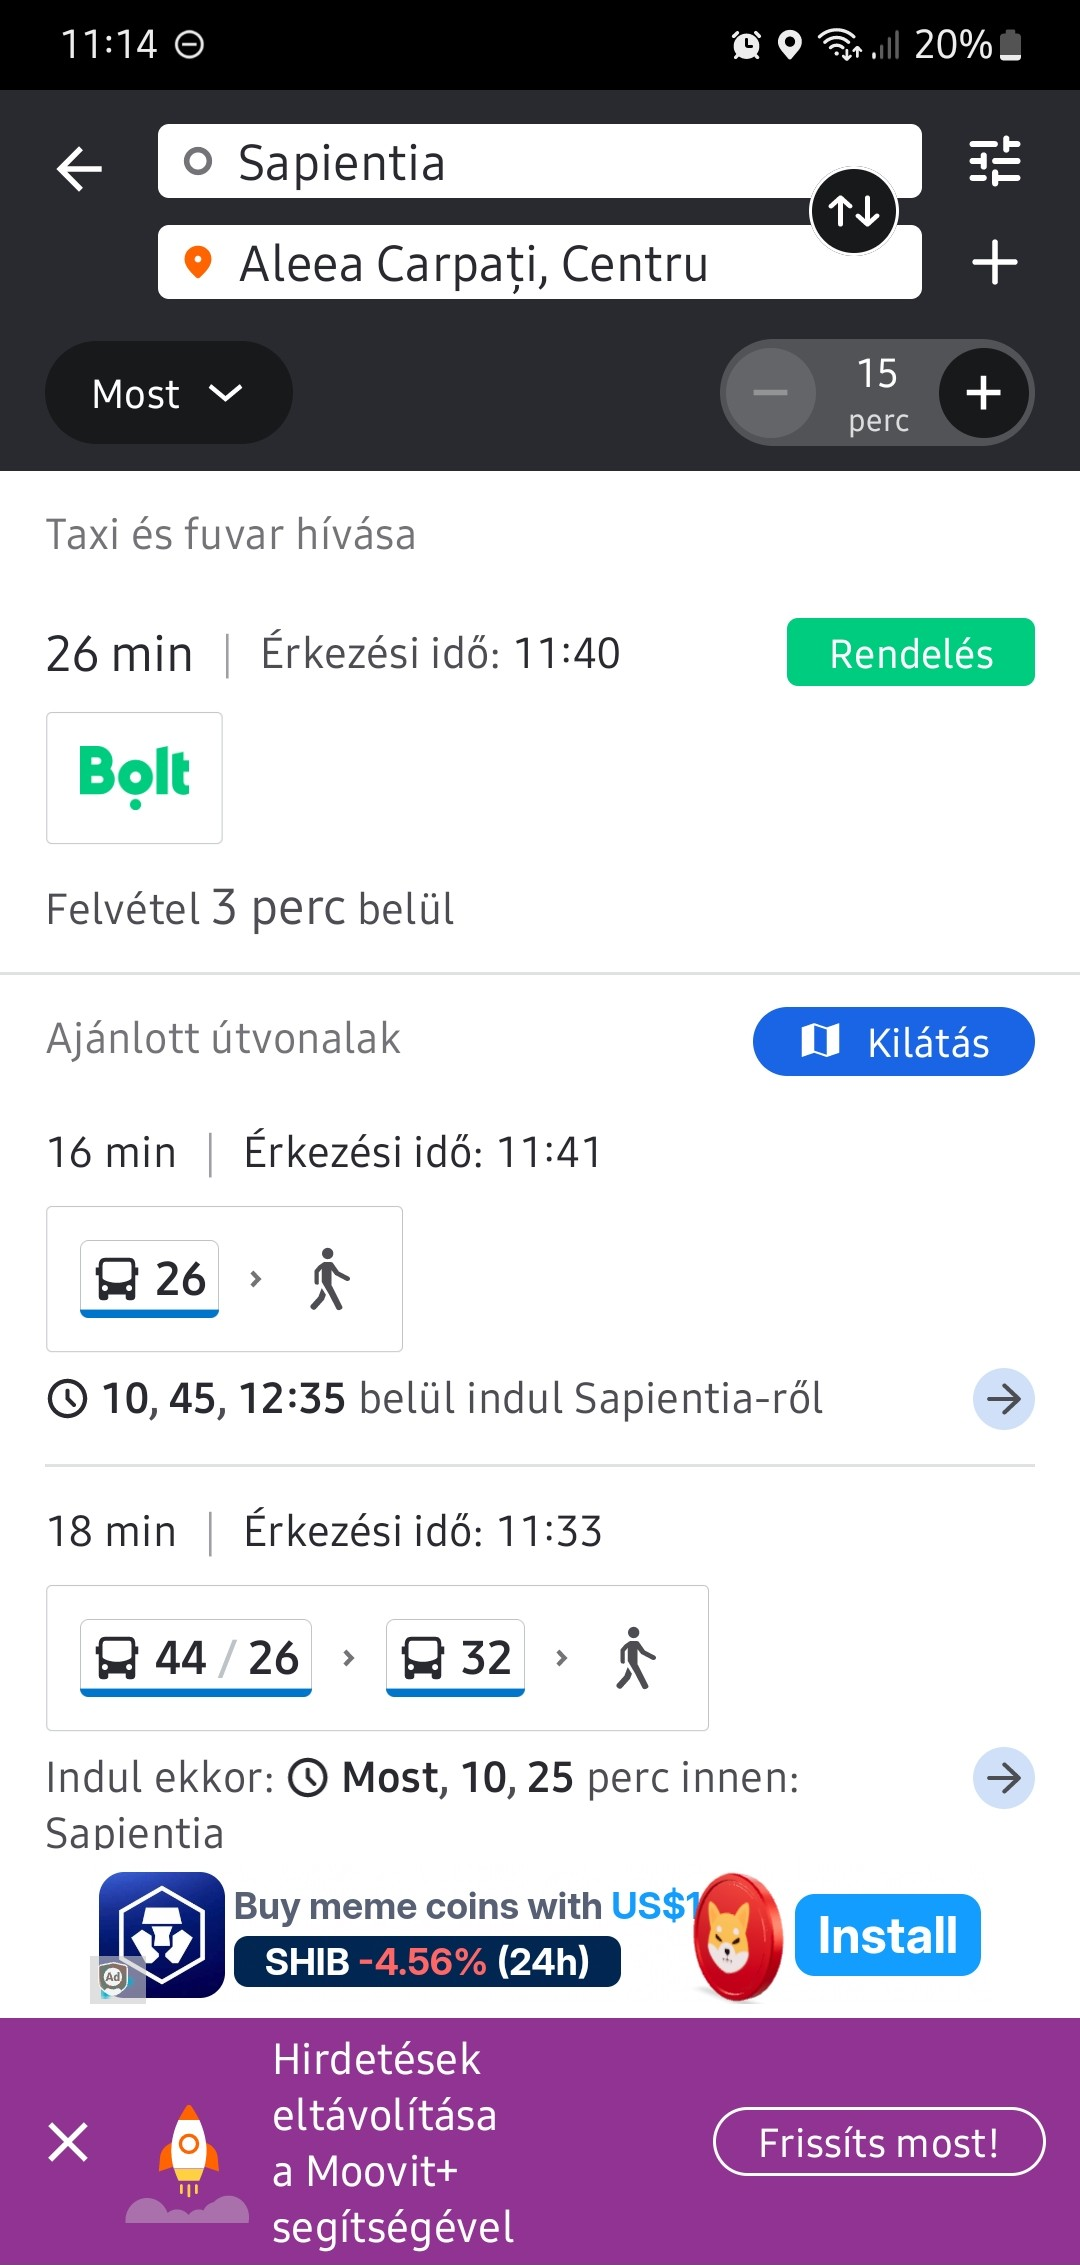
\includegraphics[width=0.275\textwidth]{figures/moovit.jpg}}
  \caption{Moovit alkalmazás}
  \label{fig:moovit}
\end{wrapfigure}

A Moovit egy népszerű alkalmazás, amely a világ számos országában és városában működik, így egy szinte mindenhol elérhető szolgáltatást nyújt, viszonylag sok funkcióval. Az alkalmazás lehetővé teszi az utasok számára, hogy megtervezzék az útvonalukat, figyelemmel kísérjék a járatokat és megvásárolják a jegyeket\footnote{Moovit: \url{https://moovit.com}}. A közlekedési információkat az utasok okostelefonjaikon futó alkalmazások biztosítják, amelyek időnként beküldik a GPS pozícióikat a Moovit szervereire. Ezenkívül a felhasználók manuálisan is megadhatnak információkat, például a járatok késéséről vagy pillanatnyi telítettségről. A rendszer ezeket az adatokat dolgozza fel és jeleníti meg a többi felhasználó számára, amennyiben ezek elegendő mennyiségben rendelkezésre állnak. Ezzel csak az a probléma hogy kevés országban éri el a felhasználók száma az elvárt szintet, így ezek a funkciók nem mindenhol érhetőek el \cite{rollandinfrastrukturalis}.

Sajnos a kevés felhasználót számláló országok közé tartozik a miénk is, így csak a hivatalosan megadott adatokat jeleníti meg a Moovit, a felhasználóktól érkezőket nem, emiatt nálunk eléggé rövid az alkalmazás által nyújtott szolgáltatások listája. Marosvásárhelyen például csak a városi buszok menetrendje és útvonala érhető el, de ehhez sem társul élő forgalmi információ és jegyvásárlási lehetőség sem. A \ref{fig:moovit} ábrán látható egy képernyőkép a Moovit alkalmazásról.

\subsection{Budapest Go}
\begin{wrapfigure}{r}{0.3\textwidth}
  \vspace{-15pt}
  \frame{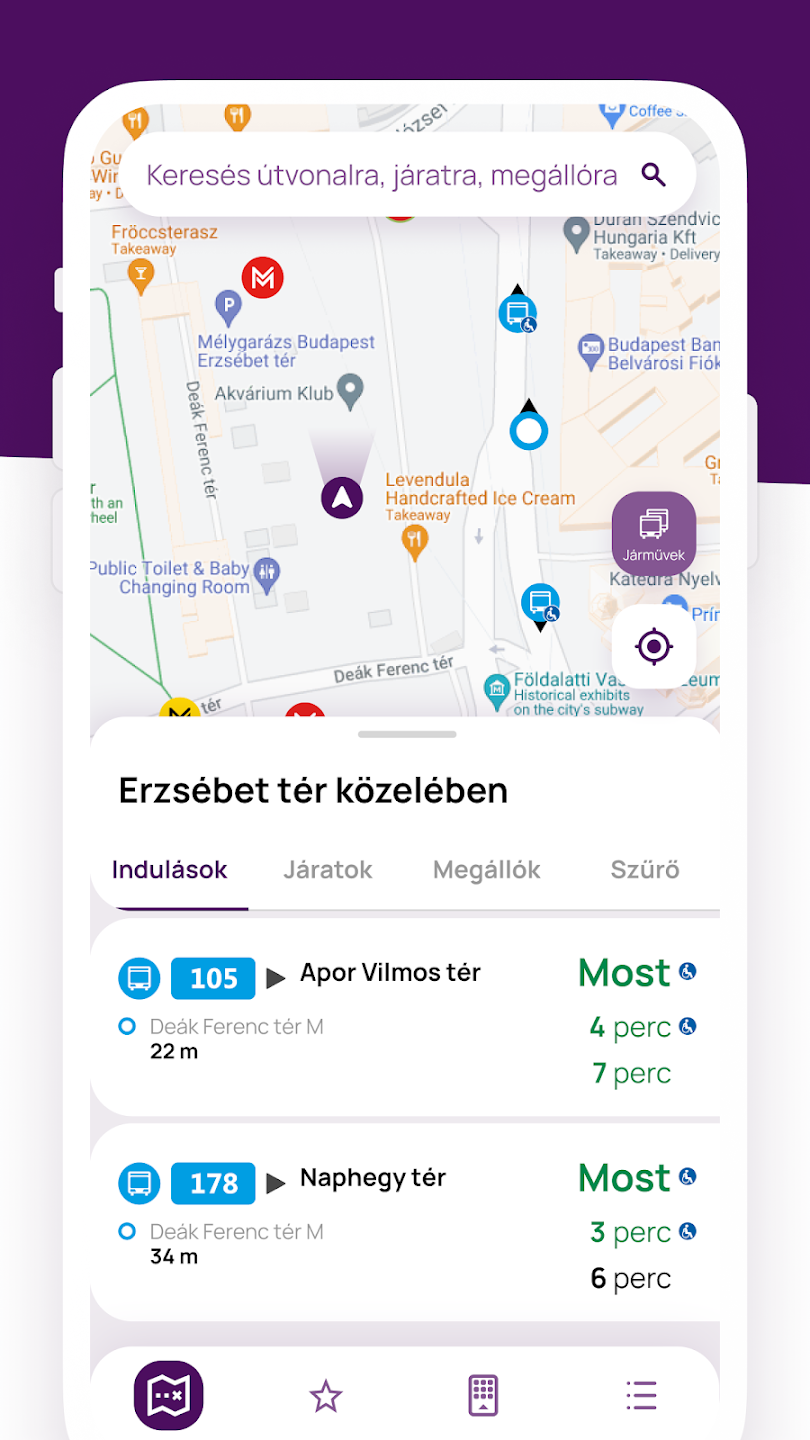
\includegraphics[width=0.3\textwidth]{figures/budapestgo.png}}
  \caption{
    \centering
    \newline
    Budapest Go alkalmazás
    \protect\footnotemark
  }
  \label{fig:budapestgo}
\end{wrapfigure}

\footnotetext{Budapest Go - Google Play Áruház: \url{https://play.google.com/store/apps/details?id=hu.webvalto.bkkfutar}}

A másik alkalmazás a Budapest Go, amely egy általános közlekedési rendszer és a városi közlekedés minden elemét lefedi, így nem csak a buszokkal való közlekedésre használható, hanem majdnem az összes tömegközlekedési eszközzel a metrótól, a villamoson át, a hajóig, sőt az egyéni közlekedés megkönnyítése végett a gyalogos- és biciklis útvonalak is megtalálhatóak benne.
Ez a megoldás talán közelebb áll a mi elképzeléseinkhez a funkcionalitás szempontjából, mert ugyanúgy biztosítja a jegyvásárlás lehetőségét, az útvonaltervezést és a valós idejű járatinformációkat, mint a Moovit, de a Budapest Go esetében ezek a funkciók sokkal részletesebbek és szélesebb körűek, emellett pedig rengeteg egyéb funkciót is biztosít. A \ref{fig:budapestgo} ábrán látható a Budapest Go alkalmazás kezdőképernyője.

Egy lényeges probléma a Budapest Go-val az, hogy nem használható fel univerzálisan, mert ez a Budapesti Közlekedési Központ (BKK) saját rendszere, ezáltal pedig Budapestre van korlátozva és csak az ottani utasok tudják kihasználni az általa biztosított szolgáltatásokat\footnote{BKK x Supercharge: All-in-one mobility solution: \url{https://supercharge.io/work/details/budapest-go}}. Ezzel szemben mi a nyitottságra szeretnénk fektetni a hangsúlyt és egy olyan rendszert hoznánk létre, amelyet bármely busztársaság tudna használni, helytől függetlenül.